%- - - - - - - - - - - - - - - - - - - - - - - - - - - - - - - - - - - -
%- - - - - - - - - - - - - - - - - - - - - - - - - - - - - - - - - - - -
%  QPLIB-3.tex
%- - - - - - - - - - - - - - - - - - - - - - - - - - - - - - - - - - - -
%- - - - - - - - - - - - - - - - - - - - - - - - - - - - - - - - - - - -
\section{Library Construction}\label{sec:lib}

In this section we present all the steps we performed in order to build
the new instance library. In \S\ref{subsec:instColl}, we describe the set
of gathered instances, and
in \S\ref{subsec:selection} we present the features used to
classify the instances.
%and discuss issues concerning the format of the instances.
We describe the selection process used to filter the instances, and
graphically present the main features of the selected instances in
\S\ref{subsec:final set}, while in \S\ref{subsec:website}
we provide information on how to access the test collection.

%- - - - - - - - - - - - - - - - - - - - - - - - - - - - - - - - - - - -
\subsection{Instance Collection}\label{subsec:instColl}

In this section we describe the procedure we adopted to gather the
instances. In January $2014$, we issued an online call for instances
using main international mailing lists of the mathematical
optimization and numerical analysis communities, reaching in this way
a \textcolor{red}{large set of possibly interested} researchers and practitioners.
The call remained open for ten months, during which we received a large
number of contributions of different nature. The instances we gathered
come both from theoretical studies as well as from real-world
applications.


In addition to these spontaneous contributions we analyzed existing generic
libraries of instances available  on the internet that contain QP
instances. Namely, the libraries from which we gathered instances are
%
\begin{itemize}
 \item the \texttt{BARON} library
 \url{http://www.minlp.com/nlp-and-minlp-test-problems};
%
\item the \texttt{CUTEst} library
 \url{https://ccpforge.cse.rl.ac.uk/gf/project/cutest};
%
\item the \texttt{GAMS Performance} libraries
 \url{http://www.gamsworld.org/performance/performlib.htm};
%
\item the \texttt{MacMINLP} library
 \url{https://wiki.mcs.anl.gov/leyffer/index.php/MacMINLP};
%
\item the \texttt{Maros-M{\'e}sz{\'a}ros} library
 \url{http://www.doc.ic.ac.uk/~im/00README.QP};
%
\item the \texttt{MINLP} library
 \url{http://www.gamsworld.org/minlp/minlplib.htm};
%
\item the \texttt{POLIP} library
 \url{http://polip.zib.de/pipformat.php}.
\end{itemize}

Other quadratic instances were found in online libraries devoted to
specific QP problems as Max-Cut, Quadratic Assignment, Portfolio
Optimization, and several others. \textcolor{red}{In addition, we mention
that other generic libraries exist, e.g., 
Conic library CBLIB (\url{http://cblib.zib.de}) and 
MIPLIB~2010 (\url{http://miplib.zib.de/}), to mention just a few.}\todo{AG: maybe cite CBLIB paper \cite{Friberg2016}}

At the end of this process we had gathered more than eight thousand
instances. Three quarters of them contained discrete variables, while
the remainder contained only continuous variables. In more detail,
we gathered $\approx 1800$ Quadratic Binary Linear (QBL) instances,
$\approx 2000$ Quadratic Continuous Quadratic (QCQ) instances,
and $\approx 2500$ Quadratic General Quadratic (QGQ) instances. We
also received $\approx 1000$ Convex General Convex (CGC) instances. We
obtained relatively fewer Quadratic Binary Quadratic (QBQ), Convex
Continuous Convex (CCC) and Convex Mixed Convex (CMC) instances,
($\approx 150$, $\approx 200$, and $\approx 200$ instances, respectively).
Finally, we found only $17$ Quadratic Mixed
Linear (QML) instances. In the call for instances, no specific format
requirements were imposed for the submissions.

To evaluate the instances we decided, for practical reasons, to use
GAMS as common platform for all our final selection computations.
%involving commercial and non-commercial solvers.
For this reason, we translated all the
instances we received into the GAMS format (\texttt{.gms}).
% In a preliminary phase, all the instances received were divided
%according to their format and subsequently translated.
%In \S\ref{subsec:tools}
%%~\ref{subsec:CP_convex}
%the tools used
%to translate an instance from a given format to the \texttt{.gms} format
%%to translate an instance from and to a given format to the
%\texttt{.gms} format
%are described in more detail.\\
%

%\subsection{Instance Features}\label{subsec:feature}

For each instance in this large starting set,
we collected important characteristics
which allowed us to classify the instances into the QP categories described in
\S\ref{sec:QPbasic}. As far as the variable types are concerned, we
collected the following information:
%
\begin{itemize}
 \item the number of binary variables; % (\emph{\# bin}),
 %
 \item the number of integer variables; and % (\emph{\# int}),
 %
 \item the number of continuous variables. % (\emph{\# cont}).
\end{itemize}
%
If at least one binary or integer variable is present, then the instance is
categorized as \emph{discrete}, otherwise it is categorized as \emph{continuous}.
As far as the objective function is concerned, we gathered the following
information:
%
\begin{itemize}
 \item the percentage of positive and negative eigenvalues of the Hessian
      $Q^0$; and
       % (\emph{\% neg eig}), and
 %
 \item the density of the Hessian $Q^0$ (number of nonzero entries divided by the total
       number of entries). %(\emph{\% dens}).
\end{itemize}
%

The number of positive (i.e., larger than $10^{-12}$) and negative (i.e., smaller than $-10^{-12}$) eigenvalues of $Q^0$ allowed us to identify the
objective function type, as in presence of at least one negative (positive) eigenvalue
the objective function is nonconvex (nonconcave). Finally, as far as the constraint types
are concerned, we collected the following information:
%
\begin{itemize}
 \item the number of linear constraints, % (\emph{\# lin}),
 %
 \item the number of quadratic constraints, % (\emph{\# quad}),
 %
 \item the number of convex constraints, and % (\emph{\# conv}),
 %
 \item the number of variable bounds (for non-binary variables). %(\emph{\# box}).
\end{itemize}
%
A constraint is considered quadratic if it contains at least one nonzero in
a quadratic term (if present). Among the quadratic constraints, the ones whose
Hessians have only non-negative eigenvalues (when $c_u^i < \infty$) and
and non-positive eigenvalues (when $c_l^i > - \infty$)
are classified as convex constraints; thus, a quadratic constraint with
two sided, finite bounds is non-convex.
Note that this might occasionally lead us to classify some instances that have conic constraints as non-convex ones, although their feasible region is in fact convex---fortunately, only some solvers are capable of properly exploiting this property.
 All this information allowed us to analyse the gathered instances and to perform the
filters described in the the next paragraph.

%- - - - - - - - - - - - - - - - - - - - - - - - - - - - - - - - - - - -
\subsection{Instance Selection}\label{subsec:selection}

During the development of the library, a discussion ensued about
the expected goals that we wished to achieve. The following four goals
where finally identified:
%
\begin{enumerate}
 \item to represent as far as possible all the different categories of QP
       problems;
 %
 \item to gather ``challenging'' instances, i.e., ones which can not be easily
       solved by  state-of-the-art solvers;
 %
 \item to include, for each of the categories, a set of well-diversified
       instances; and
 %
 \item to obtain a set of instances which is neither too small, so as to
       preserve statistical relevance, nor too large so as to being
       computationally manageable.
\end{enumerate}
%
To achieve such goals, we performed the following two filters, applied in
a cascade.
%
\begin{itemize}
 \item \emph{First Instances Filter.}\\
       The first filter was designed to drastically reduce the number of
       instances by eliminating the ``easy'' ones. An empirical measure
       for the hardness of an instance is the CPU time needed by a
       complete solver (cf.~\S\ref{sec:algo}) to solve it to
       global optimality. Accordingly, for each of the gathered instance we
       ran the complete solvers in GAMS, which number depends on the category
       of the instance under consideration, cf.~Table \ref{t:solvers}.
       We then filtered according to a first
       measure of computational difficulty, i.e., we discarded all instances
       that are solved by at least 30\% of the complete solvers within a time
       limit of 30 seconds.
 %
 \item \emph{Second Instances Filter.}\\
       The goal of the second filter was to eliminate ``similar'' instances.
       We carefully analyzed the instances one by one, and we clustered them
       according to their features; for each cluster we kept only a few
       representatives, e.g. by eliminating all but a few of those with very similar size and coming from the same donor. Finally, in order to only
       keep computationally challenging instances we ran a a complete solver for QGQ with a time limit of 120 seconds; all the
       instances which have been solved to proven optimality within this time limit
       were discarded.
\end{itemize}
%
In Table~\ref{tab:filters} we summarize the two filter steps, which
allowed us to identify the final set of $319$ discrete instances and
$134$ continuous instances.

\begin{table}
 \centering
 \setlength{\tabcolsep}{5pt}
%  \arraystretch{1}
\begin{tabular}{cccc}
Starting set& \multicolumn{ 2}{c}{ $\approx$ 8500 Instances }& \\
& \multicolumn{ 2}{c}{$\Downarrow$}& \\
& $\approx$ 6000 Discr. Inst.  & $\approx$ 2500 Cont. Inst. & \\
First Filter  & $\Downarrow$  & $\Downarrow$ & \\
 & $\approx$ 3000 Discr. Inst.  & $\approx$ 1000 Cont. Inst. & \\
Second Filter & $\Downarrow$  & $\Downarrow$  & \\
% & 600 Discr. Inst.  & 250  Cont. inst. & \\
  & 319 Discr. Inst.  & 134  Cont. inst. & \\
\end{tabular}
%\begin{center}\end{center}
\caption{Instance filter steps} \label{tab:filters}
\end{table}

%- - - - - - - - - - - - - - - - - - - - - - - - - - - - - - - - - - - -
\subsection{Analysis of the Final Set of Instances}\label{subsec:final set}

\textcolor{red}{We now analyze the features of the instances selected to be part of the
 library. In Table \ref{tab:DDDDD}, we provide a global overview. The instances have been divided in \textit{continuous} vs \textit{discrete} and \textit{convex} vs \textit{non-convex}, forming in this way, a  classification of 4 macro categories. As previously mentioned, an instance is classified \textit{discrete} if it contains at least a binary or integer variable, and \textit{continuous} otherwise. On the other hand, an instance is classified as \textit{non-convex} if the objective function is non-convex and/or at least one of the constraints is  non-convex, and \textit{convex} otherwise. }


\begin{table}
\textcolor{red}{
 \centering
 %\scriptsize
 \setlength{\tabcolsep}{18pt}
 \renewcommand \arraystretch{1.1}
\begin{tabular}{llr}
\toprule
Variables & Convexity & \#\\
\cmidrule(lr){1-3}
%
 \textit{continuous}	& \textit{convex}		&  32 \\[1.2 ex]
 \textit{continuous}	& \textit{non-convex} 	&  102 \\[1.2 ex]
 \textit{discrete}	& \textit{convex}		&  31 \\[1.2 ex]
 \textit{discrete}	& \textit{non-convex}	&  288 \\[1.2 ex]
\cmidrule(lr){1-3}
Total		&				& 453\\
%
\bottomrule
\end{tabular}
\caption{Macro classification of the final set of instances}
\label{tab:DDDDD}
}
\end{table}

 The detailed characteristics of the instances are presented in Table
\ref{tab:DD} for \emph{discrete} instances
(\textit{*}\{\textit{B,M,I,G}\}\textit{*}) and in Table
\ref{tab:CC} for \emph{continuous} ones (\textit{*C*}).
For each category, the tables
report in column ``$\#$'' the corresponding number of instances. It can be seen
that the final set well respects the original distribution of the gathered
instances among the different categories. Indeed, the discrete categories
(\textit{LMQ}) or (\textit{QBL}) are well represented by $118$ and $59$
instances, respectively. Similarly, the continuous categories
(\textit{LCQ}) and (\textit{QCQ}) are well
represented by $50$ and $17$ instances, respectively. Moreover, the library
actually covers the large majority of all possible categories of instances.

\begin{table}
 \centering
 %\scriptsize
 \setlength{\tabcolsep}{18pt}
 \renewcommand \arraystretch{1.1}
\begin{tabular}{lllr}
\toprule
Obj. Fun. & Variables & Constraints & \#\\
\cmidrule(lr){1-4}
%
\multirow{5}*{Linear}
          & \multirow{1}*{Binary}
%                    & None      &   \\
%          &         & Linear    &  \\
                    & Quadratic &   9 \\[1.2 ex]
\cmidrule(lr){2-4}
          & \multirow{2}*{Mixed}
                    & Convex    &   \textcolor{red}{14}\\[1.2 ex]
          &         & Quadratic &  \textcolor{red}{134}\\[1.2 ex]
\cmidrule(lr){2-4}
          & \multirow{1}*{Integer}
%                    & Linear    &    \\
                   & Quadratic &    2\\[1.2 ex]
\cmidrule(lr){2-4}
          & \multirow{1}*{General}
%                    & Linear    &    \\
                   & Quadratic &    3\\[1.2 ex]
\cmidrule(lr){1-4}
%\multirow{5}*{Linear}
%          & Binary  & Quadratic &   9\\
%          & \multirow{2}*{Mixed}
%                    & Convex    &   2\\
%          &         & Quadratic &  118\\
%%          & \multirow{2}*{Integer}
%%                    & Convex    &  15 \\
%%          &         & Quadratic &   5 \\
%          & {General} & Quadratic &   3 \\
%\hline
\multirow{1}*{Convex (if min)}
          & Binary  & Linear    &  \textcolor{red}{5} \\[1.2 ex]
\cmidrule(lr){2-4}
\multirow{1}*{or}
          & \multirow{2}*{Mixed}
                    & Linear    &   12\\[1.2 ex]
\multirow{1}*{Concave (if max)}
          &         & Quadratic &    \textcolor{red}{6}\\[1.2 ex]
%          & General & Linear    &    \\
%\cmidrule(lr){2-4}
%          & \multirow{1}*{Integer}
%                    & Linear    &   1\\[1.2 ex]
%\hline
\cmidrule(lr){1-4}
\multirow{6}*{Quadratic}
          & \multirow{3}*{Binary}
                    & None      &   23\\[1.2 ex]
          &         & Linear    &  \textcolor{red}{91}\\[1.2 ex]
          &         & Quadratic &   5 \\[1.2 ex]
\cmidrule(lr){2-4}
          & \multirow{2}*{Mixed}
                    & Linear    &   11\\[1.2 ex]
          &         & Quadratic &    1\\[1.2 ex]
\cmidrule(lr){2-4}
          & Integer & Linear    &    2\\[1.2 ex]
\cmidrule(lr){2-4}
          & \multirow{1}*{General}
                    & Quadratic    &    1\\[1.2 ex]
%          &         & Quadratic &    \\
\hline
Total     &         &           & \textcolor{red}{319}\\
%
\bottomrule
\end{tabular}
\caption{Classification of the final set of discrete instances}
\label{tab:DD}
\end{table}

\begin{table}
 \centering
 %\scriptsize
 \setlength{\tabcolsep}{18pt}
 \renewcommand \arraystretch{1.1}
\begin{tabular}{llr}
\toprule
Obj. Fun. & Constraints & \#\\
\cmidrule(lr){1-3}
%
\multirow{2}*{Linear}    & Convex    &   13\\[1.2 ex]
                         & Quadratic &   \textcolor{red}{52}\\[1.2 ex]
\cmidrule(lr){1-3}
\multirow{1}*{Convex (if min)}
                         & Box       &   3 \\[1.2 ex]
\multirow{1}*{or}
                         & Linear    &   \textcolor{red}{16}\\[1.2 ex]
                        % & Convex    &    2\\[1.2 ex]
\multirow{1}*{Concave (if max)}
                         & Quadratic &    \textcolor{red}{11}\\[1.2 ex]
\cmidrule(lr){1-3}
\multirow{3}*{Quadratic}
                         & Linear    &   6\\[1.2 ex]
                         & Convex    &   \textcolor{red}{3}\\[1.2 ex]
                         & Quadratic &   \textcolor{red}{30}\\[1.2 ex]
\hline
Total                    &           & \textcolor{red}{134} \\
%
\bottomrule
\end{tabular}
\caption{Classification of the final set of continuous instances}
\label{tab:CC}
\end{table}

\textcolor{red}{
One of the nontrivial choices in our library is that we made no effort to reformulate the instances, and inserted them in the library in the very same format they have been provided to us by the original contributors. Section \ref{ssec:reform} is crucial in justifying this choice, as it shows that there are several degrees of freedom to move the instances from one class to another. Tailoring the structure of a problem to the solver is, however, a bias we do not want to add.
}

We now report some graphs that help in illustrating the main features
of the instances. In Figure~\ref{fig:distribution}~(left) we plot the number
of variables (horizontal axis) versus the number of constrains
(vertical axis), both in logarithmic scale. Continuous instances are
marked with ``$+$'', and discrete ones with ``$\times$''. The figure shows
that the library contains a quite diverse set of instances in
terms of number of variables and constraints. The maximal number of constraints
is 100000, while the maximal number of
variables is almost 40000.
Figure~\ref{fig:distribution}~(right) plots the number of nonzero elements in the gradient of the objective function and the Jacobian and the number of these nonzeros corresponding to nonlinear variables, that is, it counts the appearances of variables in objectives and constraints and how often such an appearance is in a quadratic term.

%%%%%%%%%%%%%%%%%%%%%%%%%%%%%%%%%%%
\begin{figure}\centering
  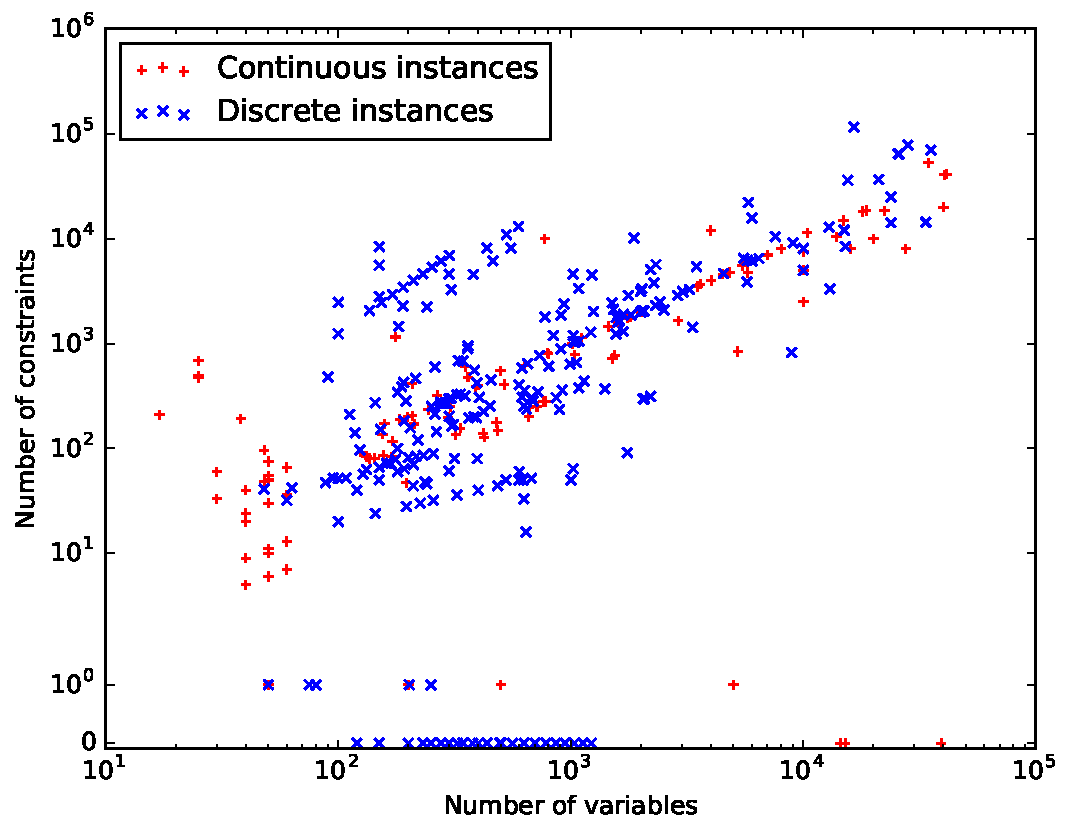
\includegraphics[width=0.50\textwidth]{pic_overview.pdf}
  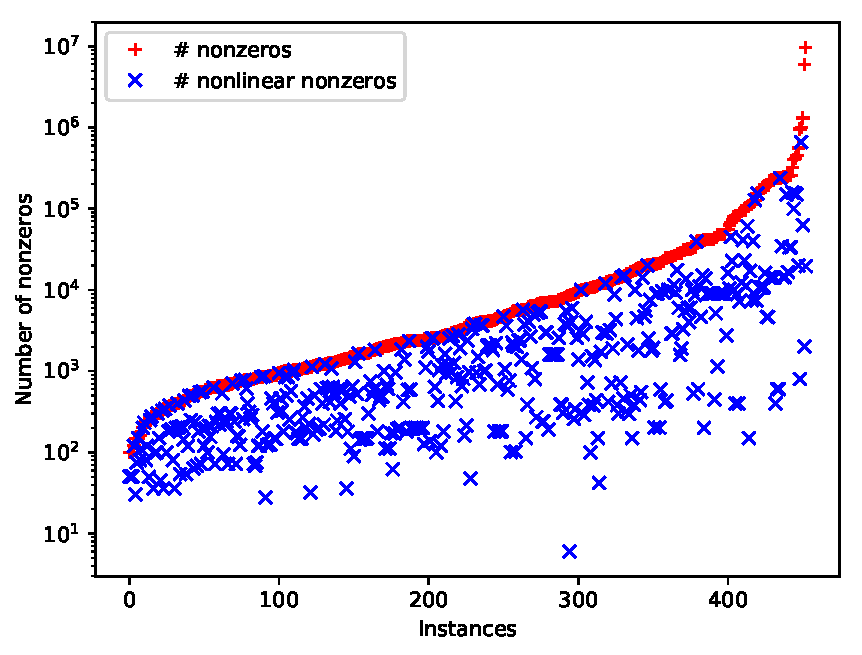
\includegraphics[width=0.49\textwidth]{pic_nz.pdf}
  \caption{Distribution of number of variables and constraints of QPLIB instances
(left). Number of (nonlinear) nonzeros of QPLIB instances (right).\label{fig:distribution}}
\end{figure}

%Figure~\ref{fig:pic_var_small}, Figure~\ref{fig:pic_var_medium} and
Figure~\ref{fig:pic_var}
describes how discrete and continuous
variables are distributed within the instances. The instances are
sorted accordingly to the total number of variables.
% and, for reason of
%readability, the graph is splitted in the three figures:
%Figure~\ref{fig:pic_var_small} describes the 100 smaller instances,
%Figure~\ref{fig:pic_var_medium} the 200 medium ones, and
%Figure~\ref{fig:pic_var_large} the 67 largest ones.
For each instance we report the total number of variables with a ``$+$'', and the total number of discrete variables (binary or general integer) with a ``$\times$''. The pictures clearly show that instances with different percentages of integer and continuous variables are present in the library, and that these differences are well distributed across the whole spectrum of variable sizes.

%%%%%%%%%%%%%%%%%%%%%%%%%%%%%%%
\begin{figure}\centering
  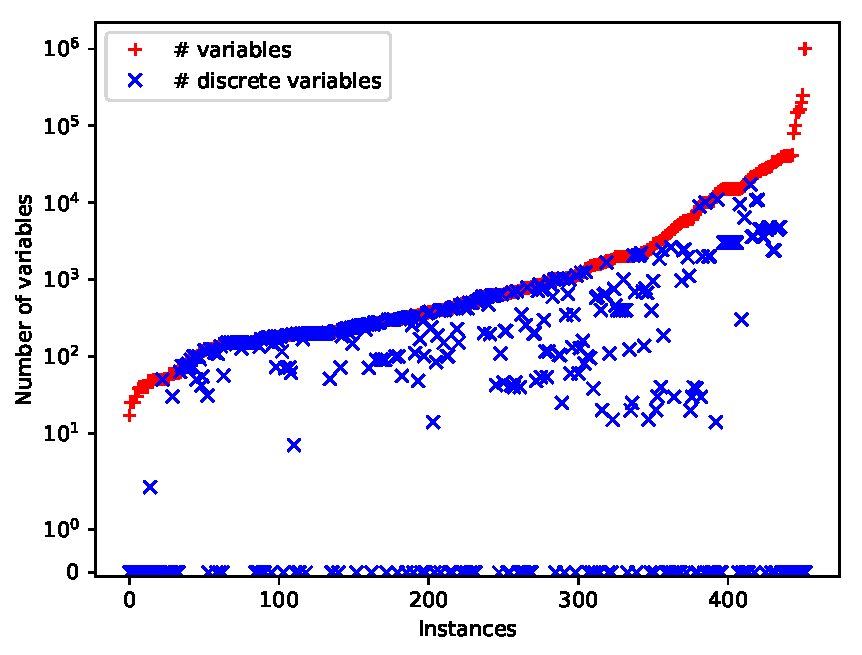
\includegraphics[width=0.55\textwidth]{pic_var.pdf}
  \caption{Number of variables of QPLIB instances. \label{fig:pic_var}}
\end{figure}

Similarly, Figure~\ref{fig:pic_constr} (left)
%Figure~\ref{fig:pic_constr_medium}
%and Figure~\ref{fig:pic_constr_big}
describes how the number of linear and quadratic
constraints are distributed within the instances. The instances are sorted
accordingly to the total number of constraints.
% and divided in the same manner as for Figures~\ref{fig:pic_var_small}--\ref{fig:pic_var_large}.
For each instance we report the total number of constraints with a ``$+$''
and the total number of quadratic constraints
with a ``$\times$''. Also, in this case, different percentages of linear and
quadratic constraints are present and well-distributed across the spectrum
of constraint sizes, although both medium- and large-size instances show a
prevalence of lower percentages of quadratic constraints. In particular,
from Figure~\ref{fig:pic_constr} (left) we learn that while the maximum number
of linear constraints exceeds 100000, the maximum number of quadratic
constraints tops up at around 10000. This is, however, reasonable, considering
how quadratic constraints can, in general, be expected to be much more
computationally challenging than linear ones, especially if nonconvex.

%%%%%%%%%%%%%%%%%%%%%%%%%%%%%%%%%%%%%%%
\begin{figure}\centering
  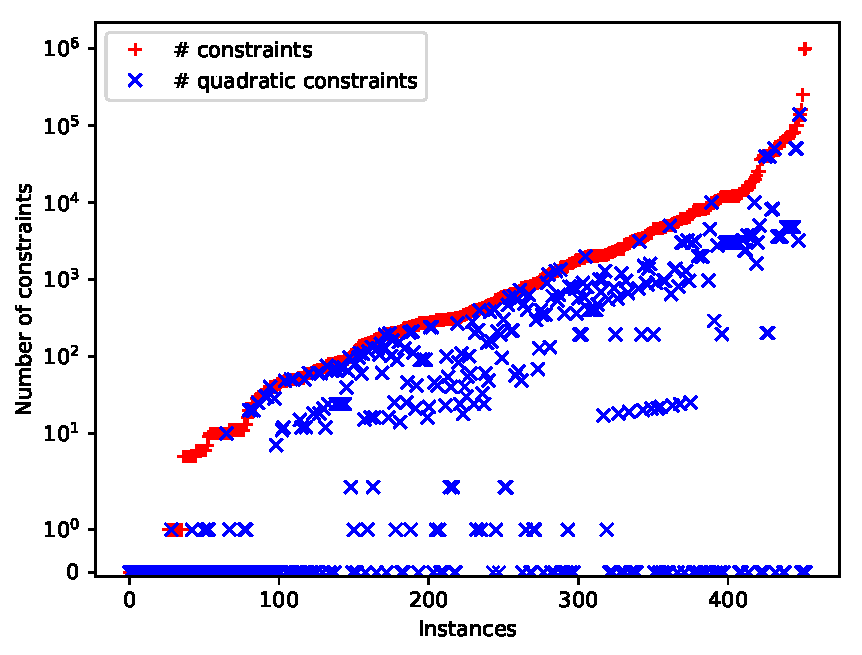
\includegraphics[width=0.49\textwidth]{pic_constr.pdf}
  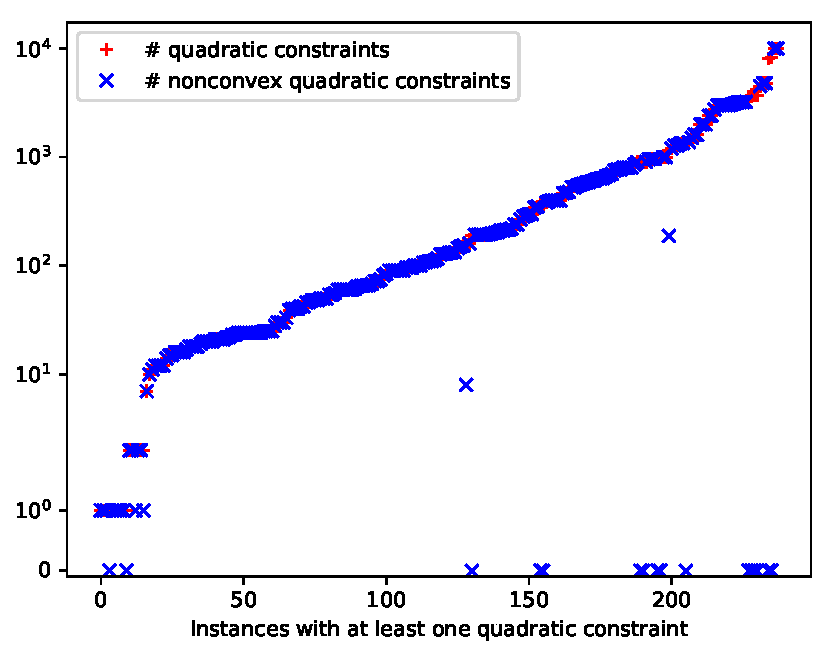
\includegraphics[width=0.49\textwidth]{pic_quad_conv_vs_nonconv.pdf}
  \caption{Number of constraints, quadratic constraints, and nonconvex quadratic constraints of QPLIB instances. \label{fig:pic_constr}}
\end{figure}

Figure~\ref{fig:pic_constr} (right) shows the instances with at least one quadratic constraint sorted according to the number of quadratic constraints (vertical axis). For each instance we report the total number of constraints with a ``$+$''
and the total number of nonconvex quadratic constraints
with a ``$\times$''.
It can be seen that the majority of instances only have nonconvex constraints. %; of those that have nonconvex ones, however, a significant fraction have no convex ones at all.




On the theme of nonconvexity, Figure~\ref{fig:pic_neg_eig} (left) focuses on
the instances with a quadratic objective function, ordered by 
 percentage of ``problematic'' eigenvalues in the Hessian $Q^0$ (vertical axis), by which
we mean \textcolor{red}{eigenvalues below $-10^{-12}$} in case of a minimization problem and \textcolor{red}{eigenvalues above $10^{-12}$} in case of a maximization problem.
The instances are mostly clustered around two values. About 25\% of the instances have a convex (if minimization) or concave (if maximization) objective function,
i.e., they have 0\% of ``problematic'' eigenvalues. Among the others, a vast
majority has around 50\% of ``problematic'' eigenvalues. However, instances
with high or low percentages of ``problematic'' eigenvalues are present, too.

\begin{figure}\centering
  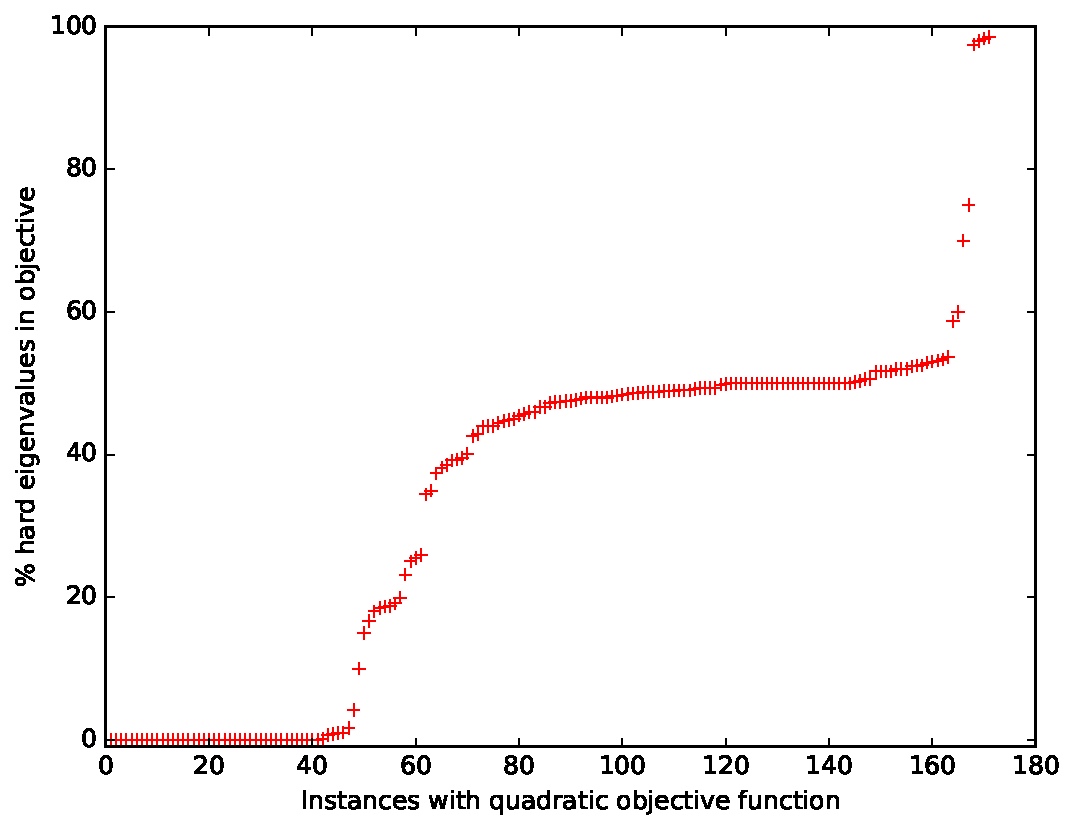
\includegraphics[width=0.49\textwidth]{pic_neg_eig.pdf}
  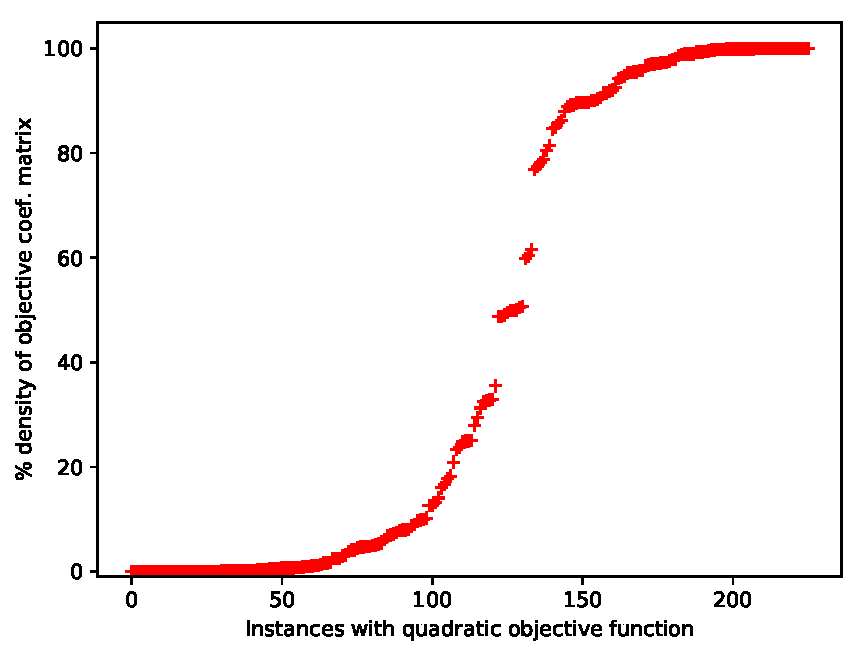
\includegraphics[width=0.49\textwidth]{pic_density.pdf}
  \caption{``Problematic'' eigenvalues (left) and density (right) of the Hessian $Q^0$ for QPLIB instances with a quadratic objective function. \label{fig:pic_neg_eig}}
\end{figure}

Similarly, Figure~\ref{fig:pic_neg_eig} (right) shows the instances with a
quadratic objective function sorted according to the density of the
Hessian $Q^0$ (vertical axis). The majority of the instances have either
a very low or a rather high density: indeed, about 30\% of the instances
have density smaller than 5\%, and about 30\% of the instances have
density larger than 50\%. However, also intermediate values are present.


Additional details on the instance features can be found in Appendix~\ref{sec:instance_details}.

%The all set of instances can be downloaded at \url{http://qplib.zib.de/html/index.html}.
%Since, as described in Section \ref{subsec:final set} the library contains instances of different nature, the website allows to filter the instances according to the classification proposed in Section \ref{ssec:taxonomy}.

\subsection{Website}\label{subsec:website}
%Select subset or categories of instances (EXTRACT FROM THE LIBRARY A SUBSET OF INSTANCES WITH SPECIFIC CHARACTERISTICS)


The QPLIB instances are publicly accessible at the website \url{http://qplib.zib.de}, which was created by extending
scripts and tools initially developed for MINLPLib\,2~\cite{Vigerske2014}.
%
We provide all instances in GAMS (\texttt{.gms}), AMPL (\texttt{.mod}), CPLEX (\texttt{.lp})
\cite{,cplex}, and  QPLIB (\texttt{.qplib}) formats. The latter is a new format
specifically for QP instances. In comparison to more \emph{high level}
formats such as \texttt{.gms} and \texttt{.lp}, the new
format offers three main advantages: it is easier to read by a stand-alone
parser (provided), it typically produces smaller files, and it permits the
inclusion of two-sided inequalities without needless repetition of data.
%the order of variables and constraints is fixed.
See Appendix~\ref{sec:format} for more details.

Beyond the instances, the website provides a rich set of metadata for
each instance: the three letter problem classification (as described in \S\ref{subsec:final set}), basic properties such as the number of variables and constraints of
different types, the sense and convexity/concavity of the objective function, and information on the nonzero structure of the
problem.
%
In addition, we display a visualization of the sparsity patterns of the Jacobian and the Hessian matrix of the
Lagrangian function.  In the plots of the Jacobian nonzero pattern, the linear and nonlinear entries are distinguished
by color.  Figure \ref{fig:sparsitypattern} shows an example for instance QPLIB\_2967.

\begin{figure}
\centering
\includegraphics[scale=0.5]{{QPLIB_2967.jac}.png} \qquad
\includegraphics{{QPLIB_2967.hess}.png}
\caption{Example for the sparsity pattern of the Jacobian of the constraint functions (left) and
  of \textcolor{red}{the upper-right triangle of} the Hessian of the Lagrangian function (right) for instance QPLIB\_2967.
  The gradient of the objective function is displayed as the first row
  of the Jacobian matrix. \textcolor{red}{Non-constant entries are shown in red.}}
\label{fig:sparsitypattern}
\end{figure}

The entire set of instances can be explored in a searchable and sortable table of selected instance features: problem
classification, convexity of the continuous relaxation, number of (all, binary, integer) variables, (all, quadratic) constraints, nonzeros, hard eigenvalues in~$Q^0$, and density of~$Q^0$.
%
Finally, a statistics page displays diagrams on the composition of the library according to different criteria: the
number of instances according to problem type, variable and constraint types, convexity, problem size, and density.
%
A file containing the relevant metadata for each instance can be downloaded in comma-separated-values (\texttt{csv}) format,
so that researchers can easily compile their own subset of instances according to these statistics.

The complete library can be downloaded as one archive, which contains the website for offline browsing and exploration.
%
In the future, we plan to extend the website by the addition of contributor information and references to the literature.



%- - - - - - - - - - - - - - - - - - - - - - - - - - - - - - - - - - - -
%- - - - - - - - - - - - - - - - - - - - - - - - - - - - - - - - - - - -
%  End QPLIB-3.tex
%- - - - - - - - - - - - - - - - - - - - - - - - - - - - - - - - - - - -
%- - - - - - - - - - - - - - - - - - - - - - - - - - - - - - - - - - - -
